\documentclass{standalone}
\usepackage{tikz}
\usepackage{ctex,siunitx}
\setCJKmainfont{Noto Serif CJK SC}
\usepackage{tkz-euclide}
\usepackage{amsmath}
\usetikzlibrary{patterns, calc,3d}
\usetikzlibrary {decorations.pathmorphing,decorations.pathreplacing,decorations.shapes}
\begin{document}
\small
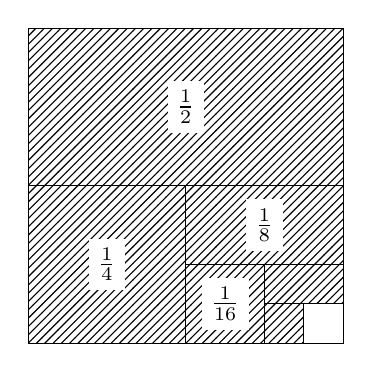
\begin{tikzpicture}[>=latex,scale=2.0]
  \draw(-1,-1)rectangle(1,1);
  \draw[pattern=north east lines](-1,0)rectangle(1,1);
  \node at (0,0.5)[fill=white]{$\frac{1}{2}$};
  \draw[pattern=north east lines](-1,-1)rectangle(0,0);
  \node at (-0.5,-0.5)[fill=white]{$\frac{1}{4}$};
  \draw[pattern=north east lines](0,-0.5)rectangle(1,0);
  \node at (0.5,-0.25)[fill=white]{$\frac{1}{8}$};
  \draw[pattern=north east lines](0,-1)rectangle(0.5,-0.5);
  \node at (0.25,-0.75)[fill=white]{$\frac{1}{16}$};
  \draw[pattern=north east lines](0.5,-0.5)rectangle(1,-0.75);
  \draw[pattern=north east lines](0.5,-0.75)rectangle(0.75,-1);
\end{tikzpicture}
\end{document}